\label{sec:training:loss}

Projector training uses bidirectional in-batch InfoNCE with Matryoshka representation learning.
For a batch of $B$ paired examples $\{(\ell_i,r_i)\}_{i=1}^{B}$, let $\mathbf{u}_i$ and $\mathbf{v}_i$ be the left and right embeddings, and let $\mathbf{u}_{i,1:k}$ denote the first $k$ dimensions.
With temperature $\tau=0.02$,
\begin{equation*}
\begin{aligned}
s_{ij}^{(k)}&=\frac{\cos(\mathbf{u}_{i,1:k},\mathbf{v}_{j,1:k})}{\tau},\\
p_{\ell\to r}^{(k)}(j|i)&=\frac{\exp(s_{ij}^{(k)})}{\sum_{m=1}^{B}\exp(s_{im}^{(k)})},\\
p_{r\to \ell}^{(k)}(j|i)&=\frac{\exp(s_{ji}^{(k)})}{\sum_{m=1}^{B}\exp(s_{mi}^{(k)})}.
\end{aligned}
\end{equation*}
\begin{equation*}
\mathcal{L}_{\mathrm{NCE}}^{(k)}=-\frac{1}{2B}\sum_{i=1}^{B}\left[\log p_{\ell\to r}^{(k)}(i|i)+\log p_{r\to \ell}^{(k)}(i|i)\right].
\label{eq:infonce}
\end{equation*}
The training loss sums this term over Matryoshka prefix dimensions,
\begin{equation*}
\begin{aligned}
\mathcal{L}&=\sum_{k\in\mathcal{K}}\mathcal{L}_{\mathrm{NCE}}^{(k)},\\
\mathcal{K}_{\mathrm{Small}}&=\{32,64,128,256,512,768,1024\},\\
\mathcal{K}_{\mathrm{Nano}}&=\{32,64,128,256,512,768\}.
\end{aligned}
\label{eq:matryoshka_loss}
\end{equation*}

We use the AdamW optimizer~\cite{adamw} with $\beta_1{=}0.9$, $\beta_2{=}0.999$, weight decay $0.01$, and global gradient clipping at $\lVert \nabla \rVert_2 \le 1$.
The learning rate is $2{\cdot}10^{-4}$ with $500$ linear warmup steps.
Training uses bf16 mixed precision and distributed data parallelism across $4$ NVIDIA H100 GPUs, with global batch size $256$ paired examples.
Projector training is run separately per modality and per task: the vision projector (\texttt{fc\_vision\_2} plus the vision modality-delimiter embeddings, where applicable) and the audio projector (\texttt{fc\_audio} plus the audio modality-delimiter embeddings) are trained in independent runs, each one using the corresponding frozen LoRA adapter inherited from Jina Embeddings v5 Text and a task-matched source mixture.
Across both model sizes, the four task variants (retrieval, classification, clustering, text-matching), and the two modalities (vision, audio), this yields $2 \times 4 \times 2 = 16$ projector-training runs in total.
Each run is trained for $15\,000$ optimizer steps.
Each batch contains examples from one source dataset sampled by mixture weight.
Figure~\ref{fig:data-distribution} summarizes the shared projector-training mixture by token share across semantic data types.
The mixture is full of text-rich and complex images like scans and diagrams, matching practical enterprise search and RAG systems that operate over real-world multimodal documents whose layout, images, and OCR/parsing stages affect retrieval quality~\cite{rag,visrag}.

\begin{figure}[H]
\centering
% Stacked bar charts of averaged sampling rates across the four task variants.
% Each row: \bar{label}{percent}{fillcolor}
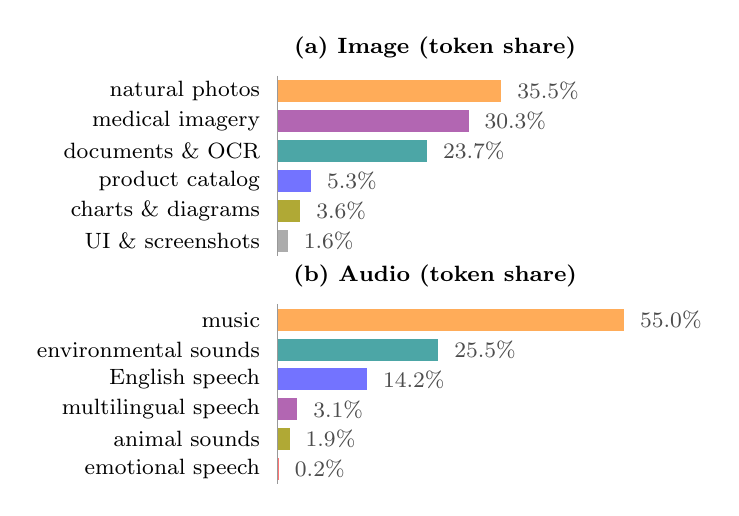
\begin{tikzpicture}[
    barlabel/.style={font=\footnotesize, anchor=east},
    barvalue/.style={font=\footnotesize, anchor=west, text=black!70},
    axisrule/.style={black!40, line width=0.4pt},
]
    \def\rowh{0.38}
    \def\scale{0.08} % 1% = 0.08 cm, so 50% = 4 cm
    \node[font=\footnotesize\bfseries] at (2.0, 0.55) {(a) Image (token share)};
    \foreach \lbl/\pct/\col [count=\i from 0] in {%
        natural photos/35.5/orange!65,%
        medical imagery/30.3/violet!60,%
        documents \& OCR/23.7/teal!70,%
        product catalog/5.3/blue!55,%
        charts \& diagrams/3.6/olive!70,%
        UI \& screenshots/1.6/gray!65%
    }{
        \pgfmathsetmacro{\y}{-\i*\rowh}
        \pgfmathsetmacro{\w}{\pct*\scale}
        \node[barlabel] at (-0.1, \y) {\lbl};
        \fill[\col] (0, \y-0.14) rectangle (\w, \y+0.14);
        \node[barvalue] at (\w+0.08, \y) {\pct\%};
    }
    \draw[axisrule] (0, 0.2) -- (0, -5.5*\rowh);

    \begin{scope}[yshift=-2.9cm]
    \node[font=\footnotesize\bfseries] at (2.0, 0.55) {(b) Audio (token share)};
    \foreach \lbl/\pct/\col [count=\i from 0] in {%
        music/55.0/orange!65,%
        environmental sounds/25.5/teal!70,%
        English speech/14.2/blue!55,%
        multilingual speech/3.1/violet!60,%
        animal sounds/1.9/olive!70,%
        emotional speech/0.2/red!55%
    }{
        \pgfmathsetmacro{\y}{-\i*\rowh}
        \pgfmathsetmacro{\w}{\pct*\scale}
        \node[barlabel] at (-0.1, \y) {\lbl};
        \fill[\col] (0, \y-0.14) rectangle (\w, \y+0.14);
        \node[barvalue] at (\w+0.08, \y) {\pct\%};
    }
    \draw[axisrule] (0, 0.2) -- (0, -5.5*\rowh);
    \end{scope}

\end{tikzpicture}

\caption{Distribution of input \emph{tokens} across semantic data types, averaged over the four task-specific checkpoints.}
\label{fig:data-distribution}
\end{figure}
